\section{基于GPU的GNN加速算法设计}
\label{sect: design}

本章节中我们将会介绍~\Mname{}的设计思路和实现细节。我们将从GNN模型的输入分析开始,接着介绍二维工作负载管理和专用内存优化,最后介绍设计优化。我们将会详细介绍每个部分的设计思路和实现细节。
\subsection{GNN模型的输入分析}
在本小节中,我们基于一个关键观察提出论点:GNN 输入信息可以指导系统优化,因为不同的 GNN 应用设置会倾向于不同的优化选择。我们介绍了两种类型的 GNN 输入信息,并讨论了它们的潜在性能优势和提取方法
\subsubsection{GNN模型信息}
尽管图神经网络的更新阶段遵循相对固定的计算模式,其聚合阶段却呈现出高度多样性。主流的图神经网络聚合方法可分为两大类型:

第一类是基于邻居节点嵌入的聚合操作(如求和、取极小值等),典型代表如图卷积网络(GCN)~\cite{GCNConv}。采用此类聚合方法的图神经网络,通常会在更新阶段(即节点嵌入矩阵与权重矩阵相乘)~\cite{GCNConv, pyG, wang2019dgl}先行降低节点嵌入维度,随后在各网络层执行聚合操作(收集邻居节点嵌入信息)。这种设计能显著减少聚合阶段的数据传输量,此时提升内存局部性将更为有利——更多节点嵌入可被缓存至高速存储器(如GPU的L1缓存),从而获得性能增益。

第二类则是需要结合特殊边特征(如权重、通过源节点与目标节点组合计算得到的边向量等)的聚合操作,如图同构网络(GIN)~\cite{GINConv}为代表。此类图神经网络必须基于完整高维节点嵌入来计算边特征。在此场景下,高速存储器(如GPU流式多处理器的共享内存)容量不足以实现有效的数据局部性优化。但考虑到计算负载可沿嵌入维度拆分并由更多并发线程共享,提升计算并行度(如基于嵌入维度的工作负载划分)反而能更有效地提高整体吞吐量。

我们通过GCN与GIN的数学表达式进一步阐释这种聚合类型差异。对于GCN,其输出嵌入$\mathbf{X}$的计算公式为:
\begin{equation}
    \mathbf{X}^{\prime} = \mathbf{\hat{D}}^{-1/2} \mathbf{\hat{A}}
    \mathbf{\hat{D}}^{-1/2} \mathbf{X} \mathbf{W},
\end{equation}
其中$\mathbf{\hat{D}}$为对角节点度矩阵,$\mathbf{W}$为权重矩阵,$\mathbf{\hat{A}}$为图邻接矩阵。而GIN每层的输出嵌入$\mathbf{X}$计算公式为:
\begin{equation}
    \mathbf{x}^{\prime}_i = h \left( (1 + \epsilon) \cdot
            \mathbf{x}_i + \sum_{j \in \mathcal{N}(i)} \mathbf{x}_j \right)    
\end{equation}
此处$h$表示神经网络(如多层感知机),负责将输入嵌入维度的节点特征$x$映射至输出嵌入维度;$\epsilon$是可根据用户需求或应用场景配置或训练的参数;$\mathcal{N}(i)$表示节点$i$的邻居集合。

假设GCN与GIN的隐藏维度均为16,输入数据集的节点嵌入维度为128。对于GCN,我们会在节点更新阶段先对节点嵌入执行基于GEMM(通用矩阵乘法)的线性变换,因此在聚合阶段仅需处理16维的节点数据。而GIN必须先在128维节点嵌入上执行邻居聚合,再通过线性变换将节点嵌入从128维降至16维。这种聚合差异导致优化策略的分化:GCN更适合对小规模节点嵌入实施内存优化,而GIN更需针对大规模节点嵌入提升计算并行度。因此,GNN的聚合类型应作为系统级优化的重要考量因素,这些信息可通过~\Mname{}内置的模型属性解析器自动获取。
\subsubsection{图信息}
\label{sect: Graph Information}
\textbf{节点度和嵌入维度:}
现实世界中的图数据通常遵循节点度的幂律分布~\cite{graph-power-law}。这种分布特性在传统图处理系统~\cite{liu2015enterprise, Mizan, han2014experimental}中已经导致工作负载不均衡问题。而在图神经网络聚合阶段,如果采用以节点为中心的工作负载划分策略,节点嵌入的高维特性会进一步加剧这种不均衡现象。更为关键的是,节点嵌入的引入使得原本适用于图处理系统的缓存优化方案失效。由于缓存容量有限(如GPU线程块的L1缓存通常为64KB),难以容纳足够数量的高维节点嵌入数据。例如,在图处理场景中,当每个节点仅含4字节浮点属性时,单个GPU线程块的L1缓存可以容纳$16\times10^3$个节点,此时时空局部性优化能带来显著性能提升。然而,对于采用64维节点嵌入的主流图神经网络而言,每个线程块仅能缓存256个节点。当处理高度节点时,系统仍需从低速全局内存中频繁获取未命中的数据,这一瓶颈严重制约了聚合阶段的执行效率。

通过获取节点度(node degree)与嵌入维度信息,我们得以基于输入数据精确估算节点工作负载及其具体构成,从而为图神经网络开辟新的优化空间。当工作负载主要受邻居节点数量主导时(例如高度节点场景),可以定制化设计并行处理更多邻居的计算方案以提升邻居间计算并行度;反之,如果工作负载主要由节点嵌入维度决定(例如高维嵌入场景),则应优先考虑沿嵌入维度增强计算并行性。需要说明的是,节点度与嵌入维度信息可直接从加载的图结构和节点嵌入向量中提取,~\Mname{}系统正是基于此类信息实现GNN工作负载的智能化管理。
。  

\textbf{图社区结构(graph community)}
~\cite{fortunato2010community, lancichinetti2008benchmark, newman2013spectral}是现实图数据的关键特征,表现为小规模节点群内部存在"强连接"(边密集),而与图其余部分仅保持"弱连接"(边稀疏)。图~\ref{fig: Graph-community}展示了利用图社区结构优化GNN的典型案例。现有图处理系统~\cite{wang2016gunrock, khorasani2014cusha}采用的节点中心聚合方案如图~\ref{fig: Graph-community}所示,各节点需先加载其邻居再独立执行聚合。当邻居仅含轻量级标量属性时,该策略可获得优异计算并行性——此时并行加载的收益足以抵消共享邻居的重复加载开销。

然而在GNN计算中,节点嵌入的高维特性使得重复加载成本成为主导因素。以节点$a$、$b$、$c$、$d$、$e$的聚合为例,传统方案需加载15个节点嵌入(其中节点$d$被$a$和$b$重复加载),且嵌入维度越高,这种冗余加载越显著。若考虑图社区结构(图~\ref{fig: Graph-community}),仅需加载5个独立节点即可完成相同聚合,有效降低内存访问量。

\begin{figure} [t]
    \centering
    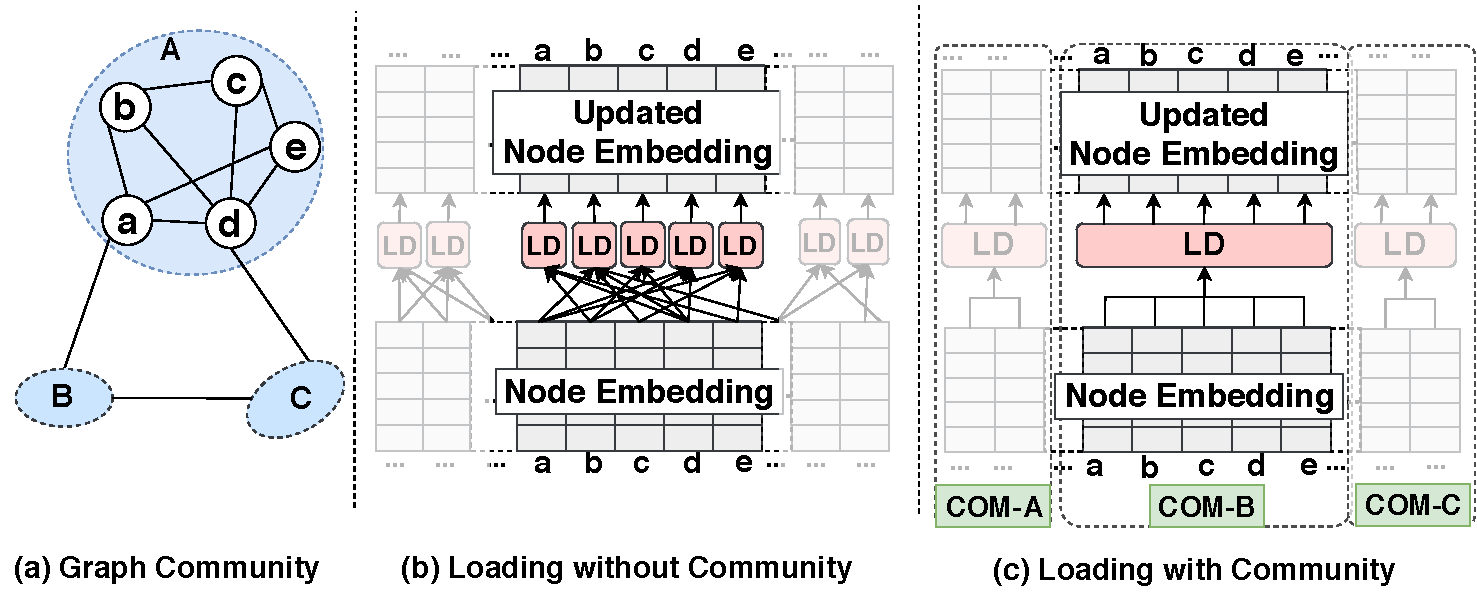
\includegraphics[width=0.98\columnwidth]{images/graph_community-1.pdf}
    \caption{图社区结构及其优化潜力(注:LD表示加载操作,COM表示社区)}
    \label{fig: Graph-community}
    \vspace{-0pt}
\end{figure}

这个想法虽然听起来很有潜力,但在GPU上的实现面临重大挑战。现有利用图社区的方法~\cite{hendrickson2000graph, newman2013spectral}主要面向CPU平台,其线程并行度有限且单线程享有MB级缓存,优化重点在于提升单线程数据局部性。而GPU具备海量并行线程但单线程仅配KB级缓存,因此关键在于通过L1缓存实现线程间数据局部性优化。具体而言需完成两个转化:将输入级的节点邻接关系转化为GPU内核级的线程、线程束和线程块邻接关系。硬件层面的核心洞见在于:相邻ID的线程更容易共享内存和计算资源,从而提升数据时空局部性。~\Mname{}通过社区感知的节点重编号和GNN专用内存优化(第\ref{sect: Specialized Memory Optimization}节)实现上述机制。
\subsection{二维工作负载管理}
\label{sect: 2D Workload Management}
图神经网络(GNN)在图计算领域占据独特地位,其核心特征在于采用高维特征向量(即嵌入表示)来表征每个节点。GNN的计算负载主要沿两个维度增长:邻居节点数量与嵌入维度规模。为此,~\Mname{}系统创新性地引入了面向GNN的输入驱动型参数化二维工作负载管理机制,该机制包含三大关键技术:粗粒度邻居分区,细粒度维度分区,线程束级线程对齐。
\subsubsection{粗粒度邻居分区}
粗粒度邻居划分是一种专为基于 GPU 的 GNN 计算设计的新颖工作负载均衡技术。它旨在解决节点间工作负载不均衡和冗余原子操作的挑战。
\begin{figure} [ht]
    \centering
    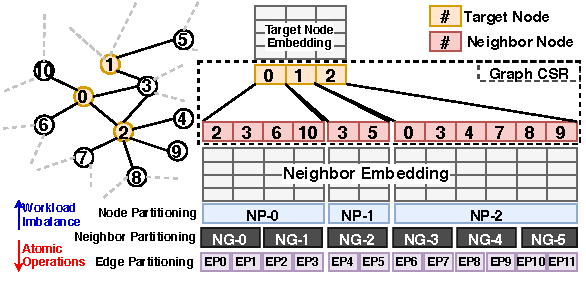
\includegraphics[width=0.9\columnwidth]{images/group-based-partitioning.pdf}
    \caption{邻居划分。注意:“NP”:节点划分;“EP”:边划分;“NG”:邻居组。}
    % \vspace{-5pt}
    \label{fig: Group-based aggregration}
\end{figure}

具体来说,基于加载的图压缩稀疏行 (CSR) 表示,我们的粗粒度邻居划分会首先将一个节点的邻居分解为一系列大小相等的邻居组,并将每个邻居组 (NG) 的聚合工作负载视为调度的基本工作负载单元。
图~\ref{fig: Group-based aggregration} 例示了一个无向图及其对应的邻居划分结果。
节点 0 的邻居被划分为两个邻居组(NG-0 和 NG-1),预定组大小为 2。节点 1 的邻居(节点 3 和节点 5)由 NG-2 覆盖,而节点 2 的邻居则分布在 NG-{3,4,5} 中。
为了支持邻居组,我们引入了两个组件:邻居划分模块和邻居划分图存储。
前者是构建在图加载器之上的一个轻量级模块,它通过将图的 CSR 划分为大小相等的组来实现。注意,为了便于调度和同步,每个邻居组仅覆盖一个目标节点的邻居。
邻居划分图存储维护每个邻居组基于元组的元数据,包括其 ID、其邻居节点在 CSR 表示中的起始和结束位置,以及源节点。例如,NG-2 的元数据将被存储为 (2, 1, (4, 6)),其中 2 是邻居组 ID,1 是目标节点 ID,(4, 6) 是 CSR 中邻居节点的索引范围。

应用基于邻居划分的聚合有以下三个好处:
1) 与基于节点/顶点中心划分的更粗粒度聚合~\cite{khorasani2014cusha}相比,邻居划分可以在很大程度上缓解工作负载单元的大小不规则性,从而提高 GPU 占用率和吞吐量性能;
2) 与更细粒度的基于边中心的划分(被现有 GNN 框架如 PyG~\cite{pyG} 用于批处理和张量化,以及被图处理系统~\cite{liu2019simd, wang2016gunrock} 用于大规模计算并行化)相比,邻居划分方案可以避免管理许多微小工作负载单元的开销,这些开销可能从多方面损害性能,例如调度开销和过多的同步操作;
3) 它引入了一个与性能相关的参数,即\textbf{邻居组大小}($ngs$),该参数用于设计参数化和性能调优。邻居划分以单个邻居节点的粗粒度进行工作。对于低维设置,它可以很大程度上缓解工作负载不均衡问题。
对于高维节点嵌入,我们采用下一小节将讨论的一种细粒度维度划分方法,将每个邻居组的工作负载进一步分发到线程。
注意,当邻居数量不能被邻居组大小整除时,会导致邻居组不均衡。
通过将邻居组大小设置为一个较小的值(例如 3),可以分摊这种不规则性。
% The choice of the neighbor group size size can also be combined with the choice of node embedding dimension for balancing the workload of each neighbor group.
% Neighbor partitioning in GNN with neighbor sampling. In the GNNs with fixed-size neighbor sampling, selecting the neighbor sample size as the neighbor group size can not show the advantage of our neighbor partitioning because even if there is no workload imbalance problem in the fixed-size sampling, it may lead to poor computing parallelism especially when the sampled neighbor size is large or the node embedding dimension is large.
% }

% \textit{Hidden dimension partitioning.} The fixed-size neighbor sampling would not change the way of dimension partitioning. For those hidden layers, each node embedding size is identical to the hidden dimension size after the neighbor aggregation and node update. Our dimension partitioning will assign a warp of 32 threads that will work on the consecutive dimension of the same neighbor group. When encountering a hidden dimension larger than one-warp of threads can cover in one iteration, we will let each thread of a warp to cover more than one dimension through iterations (Fig. 5 on Page 6). The process of hidden dimension partitioning is independent of how we determine neighbor groups with/without neighbor sampling.

% \vspace{-5pt}
\subsubsection{细粒度邻居分区}
\label{sect: Fine-grained Dimension Partitioning}
GNN 与传统图算法的区别在于其对节点嵌入的计算。
为了探索沿着这一维度加速的潜在并行性,我们利用细粒度维度划分来沿着嵌入维度进一步分配邻居组的工作负载,以提高聚合性能。
如图~\ref{fig: Dimension-based Workload Sharing.}所示,原始的邻居组工作负载被均匀地分配给 11 个连续的线程,其中每个线程独立地管理沿一个维度的聚合(即,所有邻居节点嵌入向目标节点嵌入的累加)。
如果维度大小大于工作线程的数量,则需要更多的迭代来完成聚合。

使用维度划分有两个主要原因。
首先,它可以适应更多样化的嵌入维度大小范围。
我们可以通过增加并发维度工作线程的数量或启用更多迭代来灵活地处理维度变化。
这对于具有日益复杂的模型结构和不同嵌入维度大小的现代 GNN 至关重要。
其次,它引入了另一个与性能相关的参数——用于设计定制的工作线程数量(\textbf{维度工作线程} ($dw$))。该参数的值有助于平衡线程级并行性和单线程效率(即每个线程的计算工作负载)。
\begin{figure} [t] \small
    \centering
    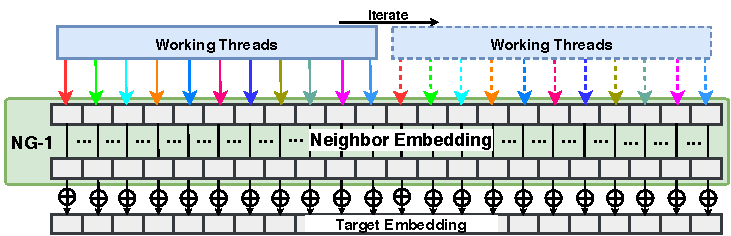
\includegraphics[width=\columnwidth]{images/dimension-sharing.pdf}
    \caption{维度划分。$\bigoplus$:累加。}
    \vspace{-15pt}
    \label{fig: Dimension-based Workload Sharing.}
\end{figure}


% \iffalse % 用户要求翻译注释掉的内容,这里暂时保留注释标记,但提供翻译
% 为了便于 ~\Mname{} 的参数选择,我们引入了两个用于性能/资源分析建模的变量,包括每个线程的工作负载(\textbf{WPT})和每个块的共享内存消耗(\textbf{SMEM})。
% \begin{equation} \small
% \label{equ: workload per threads}
% \begin{aligned}
%     \mathbf{WPT} & = ngs\times\frac{Dim}{dw} \\
%     \mathbf{SMEM} & = \frac{tpb}{tpw} \times ngs \times IntS \\
%                   &  + \frac{tpb}{tpw} \times Dim \times FloatS
% \end{aligned}
% \end{equation}
% % \fi
% 其中 $ngs$ 是邻居组大小(第~\ref{sect: Group-based Partitioning}节);$Dim$ 是节点嵌入维度;$dw$ 是维度工作线程的数量(第~\ref{sect: Fine-grained Dimension Partitioning}节);$IntS$ 和 $FloatS$ 在 GPU 上都为 4 字节。$tpb$ 是每块线程数,$tpw$ 是每 warp 线程数。对于 GPU,$tpw$ 为 32,而 $tpb$ 由用户选择。
% 为了确定 $ngs$ 和 $dw$ 的值,我们遵循两个步骤。
% 首先,我们根据 $tpw$(硬件约束)和 $Dim$(输入属性)来确定 $dw$ 的值,如公式~\ref{eq: Dimension-worker selection}所示。注意,该公式是基于跨不同数据集和 GNN 设置的大规模性能剖析得出的。
% \begin{equation} \label{eq: Dimension-worker selection}
%    dw =
%     \begin{cases}
%      tpw          &   Dim \geq tpw \\
%     \frac{{tpw}}{2} &   Dim < tpw
%     \end{cases}
% \end{equation}
% 其次,我们根据选定的 $dw$ 和 $tpb$ 来确定 $ngs$ 的值。约束条件包括使 $\mathbf{WPT} \approx 1024$ 且 $\mathbf{SMEM} \leq SMEMperBlock$。注意,$SMEMperBlock$ 在现代 GPU 上为 48 KB 到 96 KB;$tpb$ 通常选择为 2 的幂且小于或等于 1024。我们基于微基准测试和先前文献~\cite{merge-spmm}的见解表明,较小的块(1 到 3 个 warp,即 32 到 128 个线程)有利于 SM warp 调度并避免尾部效应,从而带来高 GPU 占用率和吞吐量。
% 我们在第~\ref{sect: Additional Studies}节中演示了一个分析模型的案例研究。
% \fi % 结束注释掉的内容的翻译

% Besides, we also spot the memory access pattern as a key factor to bring even better performance, since threads with continuous IDs will access to a consecutive part of memory, thus facilitating the memory coalescing on GPUs. To this end, as shown in Figure~\ref{fig: Dimension-based Workload Sharing.}\subfig{b}, we adjust the threads and their workload mapping, where adjacent threads would operate on the dimension close to each other side by side.
% % 此外,我们还发现内存访问模式是带来更好性能的关键因素,因为具有连续 ID 的线程将访问内存的连续部分,从而有助于 GPU 上的内存合并。为此,如图~\ref{fig: Dimension-based Workload Sharing.}\subfig{b}所示,我们调整了线程及其工作负载映射,使得相邻线程会并排操作彼此靠近的维度。

% \iffalse
% \begin{figure} [t] \small
%     \centering
%     \includegraphics[width=2\columnwidth]{imgs/warp-alignment.pdf}
%     % \vspace{-10pt}
%     \caption{Warp-based Thread Alignment.}
%     % (a) Unaligned-warp Execution;
%     % \todo{change the figure ... not the warp divergence. why it is always happen?}
%     % (b) Aligned-warp Execution; (c) Latency Comparison; (d) Memory Access Comparison. \todo{change the figure}}
%     % \vspace{-10pt}
%     \label{fig: warp-based Thread Alignment}
% \end{figure}
% \fi
\subsubsection{线程束级线程对齐}
虽然上述两种技术回答了我们如何逻辑地平衡 GNN 工作负载,
但是如何将这些工作负载映射到底层 GPU 硬件以实现高效执行的问题仍未解决。
一个直接的解决方案是分配连续的线程来并发处理来自不同邻居组的工作负载(图~\ref{fig: warp-based Thread Alignment})。
然而,这些线程之间不同的行为(例如,数据操作和内存访问操作)会导致线程分化和 GPU 利用率不足。
来自同一个 Warp 的线程以单指令多线程(SIMT)的方式执行,而 Warp 调度器每个周期只能处理一种类型的指令。因此,不同的线程必须等待轮到它们执行,直到流式多处理器(SM)的 Warp 调度器发出它们相应的指令。

为了应对这一挑战,我们引入了一种与我们的邻居和维度划分相协调的 Warp 对齐线程映射方法,
以系统地利用均衡工作负载带来的性能优势。
如图~\ref{fig: warp-based Thread Alignment}所示,每个 Warp 将独立管理来自一个邻居组的聚合工作负载。
因此,不同邻居组(例如,NG-0 到 NG-5)的执行可以很好地并行化,而不会引起 Warp 分化。
采用基于 Warp 的线程对齐有以下几个好处。
首先,线程间的同步(例如,原子操作)可以被最小化。同一个 Warp 的线程工作在同一个邻居组的不同维度上,因此,对于来自同一个 Warp 的线程,无论是访问全局内存还是共享内存都不会发生冲突。
% thus, no conflicts for both global and shared memory access for threads from the same warp.
% (原文注释:因此,对于来自同一个Warp的线程,全局和共享内存访问都没有冲突。)
其次,单个 Warp 的工作负载减少了,不同的 Warp 将处理更均衡的工作负载。
因此,SM Warp 调度器可以更灵活地管理更多的 Warp,以提高整体并行性。
考虑到聚合过程中每个 Warp 不可避免的全局内存访问,增加 Warp 的数量可以提高 SM 占用率以隐藏延迟。
第三,内存访问可以被合并。
来自同一个 Warp 且具有连续 ID 的线程将访问全局内存中用于节点嵌入的连续内存地址。
因此,与连续线程映射(图~\ref{fig: warp-based Thread Alignment})相比,Warp 对齐的线程映射可以将来自同一个 Warp 的内存请求合并为一个全局内存事务(图~\ref{fig: warp-based Thread Alignment})。
\begin{figure} [t] \small
    \centering
    \includegraphics[width=\columnwidth]{images/warp-alignment.pdf}
    \vspace{-15pt}
    \caption{基于 Warp 的线程对齐。}
    \vspace{-15pt}
    \label{fig: warp-based Thread Alignment}
\end{figure}
\subsection{专用内存优化}
% \vspace{-15pt}
\label{sect: Specialized Memory Optimization}
为了进一步利用二维工作负载的优势,我们引入了针对 GNN 的专用内存优化方法:\textit{社区感知的节点重编号}和\textit{Warp 感知的内存定制化}。

\subsubsection{面向社区感知的节点重编号}
\label{sect: Node Renumbering}
% Real-world graphs usually demonstrate the structure of communities~\cite{radicchi2004defining, newman2012communities, PhysRevLett.108.188701}.
% % 现实世界中的图通常表现出社区结构~\cite{radicchi2004defining, newman2012communities, PhysRevLett.108.188701}。
% Some nodes are densely connected with each other while maintaining very sparsely connections with the other nodes in the graph.
% % 一些节点彼此之间连接紧密,而与图中其他节点的连接则非常稀疏。
% Such irregularity in the edge distribution leaves a large space for locality-based optimization to improve performance.
% % 边分布的这种不规则性为基于局部性的优化以提高性能留下了很大的空间。
% In the GNNs on GPUs, nodes within each community are more likely to share the common neighbors. Therefore, caching these neighbors embeddings on the fast GPU L1 or L2 cache can reduce the redundant access to the low-speed GPU global memory.
% % 在 GPU 上的 GNN 中,每个社区内的节点更有可能共享共同的邻居。因此,将这些邻居的嵌入缓存在高速的 GPU L1 或 L2 缓存中可以减少对低速 GPU 全局内存的冗余访问。

为了探索图社区(第~\ref{sect: Graph Information}节)带来的性能优势,我们采用了轻量级的节点重编号方法,通过重新排序节点 ID 来改善 GNN 聚合过程中的时间/空间局部性,且不影响输出的正确性。
其关键思想是,节点 ID 的邻近性将映射到 GPU 上处理它们的计算单元的邻近性。
在 ~\Mname{} 中,我们的二维工作负载管理根据节点 ID 将一个节点的邻居组分配给连续的 Warp。
如果两个节点被分配了连续的 ID,
% If we assign two nodes with two consecutive numbers as their node IDs, % 如果我们将两个节点的节点ID分配为两个连续的数字,
那么它们对应的邻居组(Warp)在其 Warp ID 上也会彼此接近。
因此,它们更有可能被紧密地调度到具有共享 L1 缓存的同一个 GPU SM 上,从而提高加载的共同邻居的数据局部性。为了有效地应用节点重编号,必须解决两个关键问题。

% \vspace{-10pt}
\textbf{何时应用:} 虽然图重排序为性能提供了潜在的好处,但我们仍需弄清楚哪种类型的图能从此类重排序优化中受益。
我们的关键见解是,对于邻接矩阵已经呈现近似块对角模式形状的图(图~\ref{fig: node-renumbering}),重排序无法带来更多的局部性好处,因为每个社区内的节点在其节点 ID 方面已经彼此接近。
对于形状更不规则的图(图~\ref{fig: node-renumbering}),其边的连接以不规则模式分布在节点之间,重排序可以带来显著的性能提升(高达 2 倍加速,将在第~\ref{sect: Additional Studies}节中讨论)。
为此,我们提出了一个新的度量指标——\textit{平均边跨度}(AES),用于判断进行图重排序是否有利。
\begin{equation}  \label{equ: graph diameter}
    \mathbf{AES} = \frac{1}{\# E} \sum\limits_{(src_{id}, trg_{id}) \in E} |src_{id} - trg_{id}|
\end{equation}
其中 $E$ 是图的边集;$\#E$ 是总边数;$src_{id}$ 和 $trg_{id}$ 分别是每条边的源节点和目标节点 ID。
计算 AES 是轻量级的,并且可以在初始图加载期间动态完成。
我们对大量图进行的性能剖析也表明,当 $\sqrt{AES} > \lfloor\frac{\sqrt{\#N}}{100}\rfloor$ 时,节点重编号更有可能提高运行时性能。
\begin{figure}[htbp] % 使用 figure 环境适应单栏排版
    \centering
    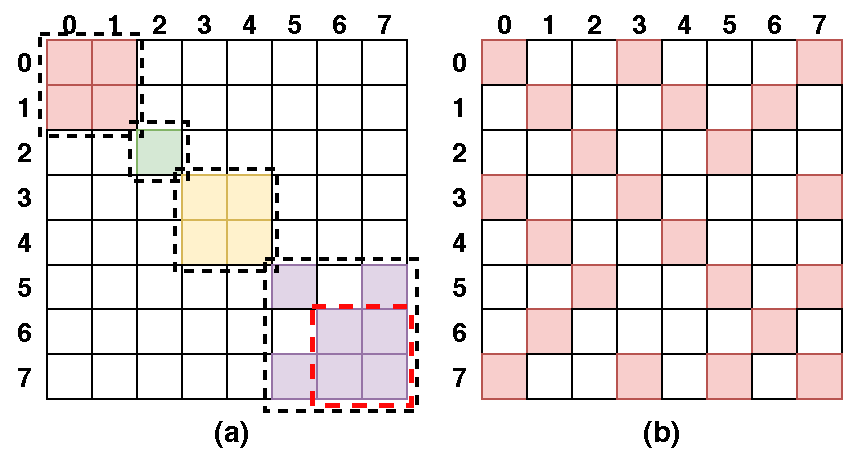
\includegraphics[width=0.6\textwidth]{images/node-renumbering.pdf} % 调整宽度为单栏的合适比例
    \vspace{-2pt} % 根据需要调整垂直间距
    \caption{图边连接模式。注意,每个彩色方块代表两个节点之间的边。(a) 中的不同颜色代表来自不同社区的边。红色虚线框表示子社区。}
    \label{fig: node-renumbering} % 修改标签以符合 LaTeX 的命名规范
    \vspace{-10pt}
\end{figure}

\textbf{如何应用:}
我们利用 Rabbit Reordering~\cite{rabbit-order}来进行重排序,这是一种完全并行化且低成本的图重排序技术。具体来说,它首先通过分层合并边和聚类节点来最大化图的模块度。然后,它通过 DFS 遍历在每个簇内生成节点顺序。
Rabbit Reordering 已经被证明在捕获的图社区质量(数据局部性)、并行化的便捷性以及性能方面优于其他图聚类方法~\cite{metis, boldi2011layered, raghavan2007near, karantasis2014parallelization, RCM-Algorithm},包括基于社区的方法(如 METIS~\cite{metis})和基于 BFS 的方法(如 Reverse Cuthill-McKee (RCM)~\cite{RCM-Algorithm})。
更重要的是,Rabbit Reordering 可以分层地捕获图社区(即,一组较小的子社区包含在一个较大的社区中,如图~\ref{fig: node-renumbering}所示例)。
这种不同粒度级别的社区能够很好地匹配 GPU 的缓存层次结构,其中较小的子社区(占用一个 SM)可以从 L1 缓存中获得数据局部性的好处,而较大的社区(占用多个 SM)可以从更大的 L2 缓存中获得数据局部性的好处。我们在第~\ref{sect: Optimization Analysis}节中定量讨论了这种局部性带来的好处。

\subsubsection{Warp 感知的内存定制化}
% In this section, we propose warp-centric shared memory customization to accelerate the aggregation operation.
% % 在本节中,我们提出以 Warp 为中心的共享内存定制化来加速聚合操作。
% As discussed earlier, the aggregation operation essentially reduces embedding vectors from multiple nodes into one vector.
% % 如前所述,聚合操作本质上是将多个节点的嵌入向量规约(reduce)成一个向量。
现有的工作~\cite{pyG, wang2016gunrock} 利用大量的全局内存访问来读取和写入嵌入,并使用大量的原子操作进行聚合(一种规约操作)。
然而,这种方法会产生巨大的开销,并且未能利用共享内存的潜在优势。
例如,当将一个具有 $k$ 个邻居组(每个组有 $ngs$ 个邻居,嵌入维度为 $Dim$)的目标节点的邻居聚合到一个 $Dim$ 维嵌入时,这涉及到 $O(k\cdot ngs\cdot Dim)$ 次原子操作和 $O(k\cdot ngs\cdot Dim)$ 次全局内存访问。

相比之下,我们提出了一种以 Warp 为中心的共享内存优化技术。
我们的关键见解是,通过根据块级 Warp 组织模式(图~\ref{fig: node-renumbering})定制共享内存布局,
% the aggregation workload among warps, each warp % (原文片段:Warp 间的聚合工作负载,每个Warp)
我们可以显著减少原子操作和全局内存访问的数量。
首先,我们为每个邻居组(Warp)的目标节点保留一个共享内存空间(对于浮点嵌入为 $4\times Dim$ 字节),这样来自一个 Warp 的线程可以将规约的中间结果缓存在共享内存中。
随后,在一个线程块内,考虑到每个节点的邻居可能分布在不同的 Warp 中,我们仅指定一个 Warp(称为\textit{领导者})负责将每个目标节点的中间结果从共享内存复制回全局内存。详细的定制化过程在算法~\ref{alg: memory-organization}中描述。
具体来说,每个 Warp(保存在 $warpPtr$ 中)具有三个属性:$nodeSharedAddr$(用于邻居组聚合结果的共享内存地址),$nodeID$(目标节点的 ID),以及 $leader$(一个布尔标志,指示当前 Warp 是否为将结果从共享内存写回到全局内存的领导者 Warp)。
主要的定制化例程(第 $4$ 行到第 $22$ 行)根据 Warp 相对于线程块的索引位置来处理不同的 Warp。
注意,这种共享内存定制化成本低廉,并且仅在 GPU 核函数执行前,与常规的图初始化过程一起动态完成一次。

在我们的设计中,当处理一个具有 $k$ 个邻居组(每个组有 $ngs$ 个邻居,嵌入维度为 $Dim$)的目标节点时,仅涉及 $O(Dim)$ 次原子操作和 $O(Dim)$ 次全局内存访问。
由此,我们可以将原子操作和全局内存访问减少 $(k\cdot ngs)$ 倍,从而显著加速聚合操作。
在这里,我们将 $ngs$ 视为一个超参数,用以平衡内存访问效率和计算并行性,我们将在第~\ref{sect: analytical modeling}节进一步讨论其值的选择。
\begin{algorithm}[htbp]
    \caption{Warp 感知的内存定制化}
    \label{alg: memory-organization}
    \begin{algorithmic}[1] \small
        \Require 邻居组大小 $\mathit{ngs}$,线程块线程数 $\mathit{threadPerBlock}$,每 Warp 线程数 $\mathit{threadPerWarp}$
        \Ensure Warp 指针数组 $\mathit{warpPtr}$
        \State $\mathit{warpNum} \gets \textbf{computeGroups}(\mathit{ngs})$ \Comment{计算邻居组数量(即 Warp 数量)}
        \State $\mathit{warpPerBlock} \gets \textbf{floor}(\mathit{threadPerBlock} / \mathit{threadPerWarp})$ \Comment{计算每个线程块的 Warp 数量}
        \State 初始化追踪变量:$\mathit{cnt} \gets 0$, $\mathit{local\_cnt} \gets 0$, $\mathit{last} \gets 0$
        \While{$\mathit{cnt} < \mathit{warpNum}$}
            \If{$\mathit{cnt} \bmod \mathit{warpPerBlock} == 0$} \Comment{位于线程块起始位置的 Warp}
                \State $\mathit{warpPtr[cnt].nodeSharedAddr} \gets \mathit{local\_cnt} \times \mathit{Dim}$
                \State $\mathit{last} \gets \mathit{warpPtr[cnt].nodeID}$
                \State $\mathit{warpPtr[cnt].leader} \gets \textbf{true}$
            \Else
                \If{$\mathit{warpPtr[cnt].nodeID} == \mathit{last}$} \Comment{Warp 的目标节点与前一个 Warp 相同}
                    \State $\mathit{warpPtr[cnt].nodeSharedAddr} \gets \mathit{local\_cnt}$
                \Else \Comment{Warp 的目标节点与前一个 Warp 不同}
                    \State $\mathit{local\_cnt} \gets \mathit{local\_cnt} + 1$
                    \State $\mathit{warpPtr[cnt].nodeSharedAddr} \gets \mathit{local\_cnt}$
                    \State $\mathit{last} \gets \mathit{warpPtr[cnt].nodeID}$
                    \State $\mathit{warpPtr[cnt].leader} \gets \textbf{true}$
                \EndIf
            \EndIf
            \If{$(++\mathit{cnt}) \bmod \mathit{warpPerBlock} == 0$} \Comment{下一个 Warp 属于新的线程块}
                \State $\mathit{local\_cnt} \gets 0$
            \EndIf
        \EndWhile
    \end{algorithmic}
\end{algorithm}
\subsection{设计优化}
\label{sect: analytical modeling}
\vspace{-5pt}
我们 GPU 核函数配置中的参数可以进行调整,以适应各种 GNN 模型和图数据集。
但是,如何自动选择能够带来最优性能的参数仍然是一个未知的问题。
在本节中,我们介绍 ~\Mname{} 中 \textbf{Decider}(决策器)所使用的分析模型和自动参数选择方法。

\textbf{分析建模:}
~\Mname{} 的性能/资源分析模型有两个变量:每个线程的工作负载 ($\mathit{WPT}$) 和每个块的共享内存使用量 ($\mathit{SMEM}$)。
\begin{equation} 
\label{equ: workload per threads}
    \begin{aligned}
        \mathbf{WPT}  = \mathit{ngs}\times\frac{Dim}{\mathit{dw}}, \ \
        \mathbf{SMEM}  =  \frac{\mathit{tpb}}{\mathit{tpw}} \times Dim \times \mathit{FloatS}
    \end{aligned}
\end{equation}
其中 $\mathit{ngs}$ 和 $\mathit{dw}$ 分别是邻居组大小和维度工作线程数量(第~\ref{sect: Fine-grained Dimension Partitioning}节);
$\mathit{Dim}$ 是节点嵌入维度;
$\mathit{IntS}$ 和 $\mathit{FloatS}$ 在 GPU 上均为 4 字节;
$\mathit{tpb}$ 是每块线程数,$\mathit{tpw}$ 是每 Warp 线程数;
对于 GPU,$\mathit{tpw}$ 为 32,而 $\mathit{tpb}$ 由用户选择。

\textbf{参数自动选择:}
为了确定 $\mathit{ngs}$ 和 $\mathit{dw}$ 的值,我们遵循两个步骤。
首先,我们根据 $\mathit{tpw}$(硬件约束)和 $\mathit{Dim}$(输入属性)来确定 $\mathit{dw}$ 的值,如公式~\ref{eq: Dimension-worker selection}所示。
注意,我们是通过对不同数据集和 GNN 模型进行性能剖析来得出这个公式的。
\begin{equation} \label{eq: Dimension-worker selection}
   \mathit{dw} =
    \begin{cases}
     \mathit{tpw}          &   \mathit{Dim} \geq \mathit{tpw} \\
    \frac{\mathit{tpw}}{2} &   \mathit{Dim} < \mathit{tpw}
    \end{cases}
\end{equation}
其次,我们根据选定的 $\mathit{dw}$ 和用户指定的 $\mathit{tpb}$ 来确定 $\mathit{ngs}$ 的值。
约束条件包括使 $\mathit{WPT} \approx 1024$ 且 $\mathit{SMEM} \leq \mathit{SMEMperBlock}$。注意,$SMEMperBlock$ 在现代 GPU 上为 48KB 到 100KB~\cite{rtx-4060}。
在不同的 GPU 上,即使 CUDA 核心数量和全局内存带宽不同,单线程的工作负载能力(由 $\mathit{WPT}$ 衡量)仍然相似。
$\mathit{tpb}$ 通常选择为 2 的幂且小于或等于 1024。
我们基于微基准测试和先前文献~\cite{merge-spmm}的分析表明,较小的块(1 到 4 个 Warp,即 $32 \leq \mathit{tpb} \leq 128$)可以提高 SM Warp 调度的灵活性并避免尾部效应,从而带来更高的 GPU 占用率和吞吐量。
我们将在第~\ref{sect: Additional Studies}节进一步证明我们分析模型的有效性。

% \iffalse
% % We are also considering several aspects in our design optimizations.
% % % 我们在设计优化中也考虑了几个方面。
% % \todo{Q: Why GNN input information can be used to reliably estimate GNN workloads?}
% % % % 问题:为什么 GNN 输入信息可以用来可靠地估计 GNN 工作负载?
% %
% % First, our workload/resource estimation considers the most basic computation blocks in GNNs. Modern GNN model variants are built with the same set of computation blocks but just in different ways of organizations (\textit{e.g.}, the number of blocks and their inter-connection sequence) and configurations (e.g., hidden dimension of each block). Therefore, we believe our estimation can reliably handle the modern GNNs with different model architectures.
% % % % 首先,我们的工作负载/资源估计考虑了 GNN 中最基本的计算块。现代 GNN 模型变体是使用相同的计算块集构建的,只是组织方式(例如,块的数量及其互连顺序)和配置(例如,每个块的隐藏维度)不同。因此,我们相信我们的估计能够可靠地处理具有不同模型架构的现代 GNN。
% % %
% % Second, our profiling scheme includes two key features to handle unseen GNNs. 1) it uses synthesized data to cover a full range of different possible input settings. 2) the profiling is done for the basic computation blocks instead of a complete GNN model. As argued above, this should generalize to modern architectures.
% % % % 其次,我们的性能剖析方案包含两个关键特性来处理未见过的 GNN。1) 它使用合成数据来覆盖各种可能的输入设置。2) 性能剖析是针对基本计算块而不是完整的 GNN 模型进行的。如上所述,这应该能推广到现代架构。
% % \todo{Q: Support for more schemes like full-batch or cluster-batch training, sampled neighborhoods, sampled neighborhoods}
% % % % 问题:是否支持更多方案,如全批量(full-batch)或簇批量(cluster-batch)训练,邻居采样?

% % Our current framework supports full-batch and cluster-batch training, and we demonstrate the evaluation of full-batch cases (Section~\ref{sect: compared with DGL}).
% % % % 我们当前的框架支持全批量和簇批量训练,并且我们展示了全批量情况的评估(第~\ref{sect: compared with DGL}节)。
% % Neighbor sampling is not supported by the current framework, but we see no technical challenges to add such functionality.
% % % % 当前框架不支持邻居采样,但我们认为添加此功能没有技术挑战。
% % The following gives our reasoning:
% % % % 以下是我们的理由:
% % 1) We will need to incorporate an efficient implementation to do sampling on GPUs for these sampled GNNs, but fortunately this functionality has been well studied in traditional graph analytics frameworks, such as the random walk engine~\cite{KnightKing};
% % % % 1) 对于这些采样 GNN,我们需要集成一个高效的 GPU 采样实现,但幸运的是,该功能在传统图分析框架中已有充分研究,例如随机游走引擎~\cite{KnightKing};
% % 2) The key change here is the workload estimation. Obviously, using node degree as input information only is not appropriate anymore, instead, we need to consider the neighbor sample rate to estimate the workload more accurately since in this case not all neighbors of a vertex are involved in the GNN computation. We believe all other optimizations still work in a similar way and the performance improvement would still be significant, as the computation overhead is still on the neighbor aggregation for these sampled GNNs.
% % % % 2) 这里的关键变化是工作负载估计。显然,仅使用节点度作为输入信息已不再合适,我们需要考虑邻居采样率来更准确地估计工作负载,因为在这种情况下,并非顶点的所有邻居都参与 GNN 计算。我们相信所有其他优化仍然以类似的方式工作,性能提升仍将是显著的,因为对于这些采样 GNN,计算开销仍然在于邻居聚合。
% \fi
\subsection{本章小结}

本章详细阐述了面向 GPU 的高性能图神经网络(GNN)加速算法框架 \Mname{} 的设计理念与关键技术实现。针对 GNN 计算中存在的计算模式多样性、工作负载不均衡以及高维嵌入带来的内存访问瓶颈等核心挑战,本章从 GNN 输入特性分析出发,提出了一系列优化策略。
首先,本章分析了 GNN 模型信息(聚合类型)和图信息(节点度、嵌入维度、社区结构)对优化策略选择的指导意义,强调了基于输入信息进行自适应优化的重要性。
其次,为应对 GNN 计算负载在邻居数量和嵌入维度上的双重增长特性,\Mname{} 创新性地引入了二维工作负载管理机制。该机制包含:1) 粗粒度邻居分区,通过将邻居划分为固定大小的邻居组(NGs),有效缓解了节点间工作负载不均衡,并引入了可调参数 ngs;2) 细粒度维度分区,将邻居组的计算任务沿嵌入维度分发给多个线程(dw),提升了计算并行度以适应不同嵌入维度;3) 线程束级线程对齐,将每个邻居组的聚合任务映射到一个独立的 Warp,最大限度地减少了 Warp 内分化,降低了同步开销,并改善了内存访问合并效率。
再次,为了进一步挖掘性能潜力并利用图数据的内在结构,本章提出了专用内存优化技术:1) 社区感知的节点重编号,利用轻量级图重排序算法(如 Rabbit Reordering)和平均边跨度(AES)度量,在预处理阶段优化节点ID布局,增强了计算过程中的数据时空局部性,尤其是在具有明显社区结构或边分布不规则的图上效果显著;2) Warp 感知的内存定制化(详见算法~\ref{alg: memory-organization}),通过为每个 Warp 分配目标节点的共享内存缓冲,并指定 Leader Warp 负责最终结果写回,显著减少了聚合过程中的原子操作和全局内存访问次数,大幅降低了内存开销。
最后,为了实现算法参数的自动化配置,本章介绍了 \Mname{} 内置决策器(Decider)所采用的分析模型与参数自动选择方法。通过建立工作负载(WPT)和共享内存(SMEM)的量化模型,并结合硬件约束与输入特性,该方法能够自动推导出较优的邻居组大小(ngs)和维度工作线程数(dw),从而简化了用户配置,并确保了算法在不同 GNN 模型和数据集上的高效执行。
综上所述,本章提出的 \Mname{} 设计,通过对 GNN 输入信息的深刻洞察、创新的二维工作负载管理、以及针对性的专用内存优化和自动化参数调优,构建了一套系统性的 GNN 加速方案,旨在显著提升 GNN 在 GPU 平台上的训练与推理性能。
